\begin{problem}{}{}{}{0.5 секунды}{64 Мб}
% Тетрис - Уровень 9

Помните как Коля узнал о том, что Тетрис станет культовой игрой в будущем? Чтобы дойти по девятого
уровня игры, Коля начал с нулевого, и вам тоже стоит!

{\bf {Тетрис}} "-- компьютерная игра, первоначально изобретённая и разработанная советским
программистом Алексеем Пажитновым. Игра была выпущена 6 июня 1984 года "-- в это время Пажитнов
работал в Вычислительном центре Академии наук СССР.

Тетрис представляет собой головоломку, построенную на использовании геометрических фигур
<<тетрамино>> "-- разновидности полимино, состоящих из четырёх квадратов.

\begin{wrapfigure}{r}{0.35\textwidth}
\vspace{-20pt}
  \begin{center}
    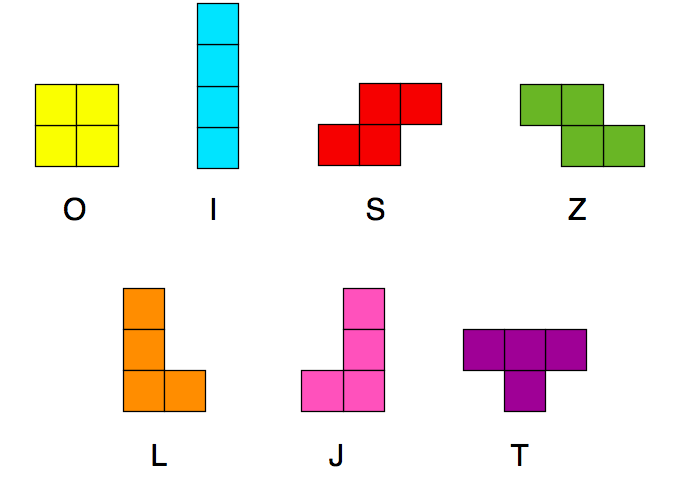
\includegraphics[width=0.35\textwidth,natwidth=267,natheight=200]{tetromino.png}
  \end{center}
  \vspace{-20pt}
  \vspace{1pt}
\end{wrapfigure}

Конечно же в 2084 году в компьютерные игры играют роботы, а не люди, поэтому и вместо
привычного клавиатурного управления игра была адаптирована для команд роботов.

{\bf {Правила игры}}

Случайные фигурки тетрамино падают сверху в прямоугольный стакан шириной 10 и высотой 20 клеток.
Как только появляется тетрамино, робот-игрок может повернуть фигурку на 90\textdegree и сдвинуть её
по горизонтали, после чего тетрамино летит вниз до тех пор, пока не наткнётся на другую фигурку
либо на дно стакана. Если при этом заполнился горизонтальный ряд из 10 клеток, он пропадает и всё,
что выше него, опускается на одну клетку.

Для того чтобы выиграть в Тетрис на 9 уровне достаточно сократить 10 строк.

Для того чтобы управлять тетрамино у роботов есть три команды: <<shift_left>> (сдвинуть влево),
<<shift_right>> (свдинуть вправо) и <<rotate>> (повернуть на 90\textdegree по часовой стрелке с
сохранением позиции относительно левого края стакана).

\InputFile
В каждой новой строке входного потока данных игра будет сообщать через пробел тип
тетрамино (одна заглавная буква английского алфавита: <<O>>, <<I>>, <<S>>, <<Z>>, <<J>>, <<L>>,
<<T>>) и начальную позицию относительно левого края стакана (индексация с 1). Тетрамино всегда
повёрнуты одинаково, как изображены на картинке выше.

Игра сообщит число 0, когда вы проиграете или наберёте достаточное количество очков.

\OutputFile
На каждую строку ввода с указанием позиции очередного тетрамино программа должна сообщить набор
команд, разделённых пробелом.

Если вы выведете некорректную команду, вы получите ответ PE; если вы проиграете раньше чем
сократите 10 строк, вы получите WA.

\Example

\begin{example}
\exmp{I 4

O 3

I 5

I 7

I 3

0
}{shift_left shift_left shift_left rotate

shift_right shift_right

rotate shift_right shift_right

rotate

rotate shift_left shift_left
}%
\end{example}

\Note
Задача не имеет однозначного ответа и оценивание будет проводиться по итогу нескольких игр, 
поэтому представленный вариант ответа "-- это лишь один из сотен возможных вариантов.

Первое тетрамино квадратной формы <<I>> (вертикальная прямая) появилось с отступом в 4 клетки
от левого края и мы решили сдвинуть его влево до упора и повернуть горизонтально; вторым
тетрамино было формы <<O>> (квадрат) появилось с отступом в 3 клетки и мы сдвинули
его в центр; третье (<<I>>) мы повернули и передвинули до упора вправо, тем самым сократив
первую строчку; четвёртое (<<I>>) мы только поворачиваем, так оно занимает клетки 7-10 на дне
стакана; пятое (<<I>>) мы поворачиваем и двигаем до упора влево и сокращаем вторую строку.
Для краткости примера мы остановили игру на этом шаге, получив от игры число 0.

Обратите внимание, игра не будет давать вам позицию следующего тетрамино пока вы не выведете
действия к текущему тетрамино!

\end{problem}

